\begin{thebibliography}{1}
\bibitem{infineon_lna}
Infineon Technologies AG: \emph{BFR181W Silicon NPN RF Transistor}, Datenblatt, 2017. Online verfügbar unter: \url{https://ilias3.uni-stuttgart.de/ilias.php?baseClass=ilrepositorygui&cmdNode=z5:o1&cmdClass=ilObjFileGUI&cmd=sendfile&ref_id=4067156} (zugegriffen am 19.05.2025)

\bibitem{hf-Verstaerker}
Advanced Test Equipment Corp.: \emph{What is an RF Amplifier?}, o.J.. Online verfügbar unter: \url{https://www.atecorp.com/solutions/what-is-an-rf-amplifier} (zugegriffen am 17.05.2025)

\bibitem{hf-Verstaerker2}
Wikipedia: \emph{Verstärker (Elektrotechnik)}, o.J.. Online verfügbar unter: \url{https://de.wikipedia.org/wiki/Verst%C3%A4rker_(Elektrotechnik)} (zugegriffen am 17.05.2025)

\bibitem{SParrameter}
Denisowski, Paul: \emph{S-Parameter verstehen}. In: Rohde \& Schwarz GmbH \& Co. KG, o.J.. Online verfügbar unter: \url{https://www.rohde-schwarz.com/de/produkte/messtechnik/essentials-test-equipment/spectrum-analyzers/s-parameter-verstehen_257831.html#gallery-7} (zugegriffen am 18.05.2025)

\bibitem{SchaltplanPCBV4}
Simon Haussmann: \emph{Schaltplan\_PCB\_V4}, 15. April 2024. In: Institut für Robuste Leistungshalbleitersysteme, Universität Stuttgart. Online verfügbar unter: \url{https://ilias3.uni-stuttgart.de/ilias.php?baseClass=ilrepositorygui&cmdNode=z5:o1&cmdClass=ilObjFileGUI&cmd=sendfile&ref_id=4067155} (zugegriffen am 19.05.2025)


\bibitem{UnderstandingSmithChart}
Denisowski, Paul: \emph{Understanding the Smith chart}. In: Rohde \& Schwarz GmbH \& Co. KG, o.J.. Online verfügbar unter: \url{https://www.rohde-schwarz.com/uk/products/test-and-measurement/essentials-test-equipment/spectrum-analyzers/understanding-the-smith-chart_257989.html#} (zugegriffen am 19.05.2025)

\bibitem{Arbeitspunk}
Schnabel, Patrick: \emph{Arbeitspunkteinstellung}. In: Elektronik-Kompendium Online verfügbar unter: \url{https://www.elektronik-kompendium.de/sites/slt/1506301.htm} (zugegriffen am 20.05.2025)

\bibitem{Reflexionsfaktor}
Ruppert, Klaus: \emph{Reflexionsfaktor}. In: Wikipedia Online verfügbar unter: \url{https://de.wikipedia.org/wiki/Reflexionsfaktor} (zugegriffen am 20.05.2025)

\bibitem{Kalibrierung}
Dr.  Latzel, Georg: \emph{SOLT Kalibrierung}. In: dl6gl Amateurfunk : \url{https://dl6gl.de/vnwa-kalibrierung.html} (zugegriffen am 20.05.2025)

\bibitem{NT-Skript}
Prof. Jan Hesselbarth: \emph{Allgemein Wissen}. In: Nachrichtentechnik 1 : \url{Nachrichtentechnik 1 Skript} (zugegriffen am 20.05.2025)

\end{thebibliography}

%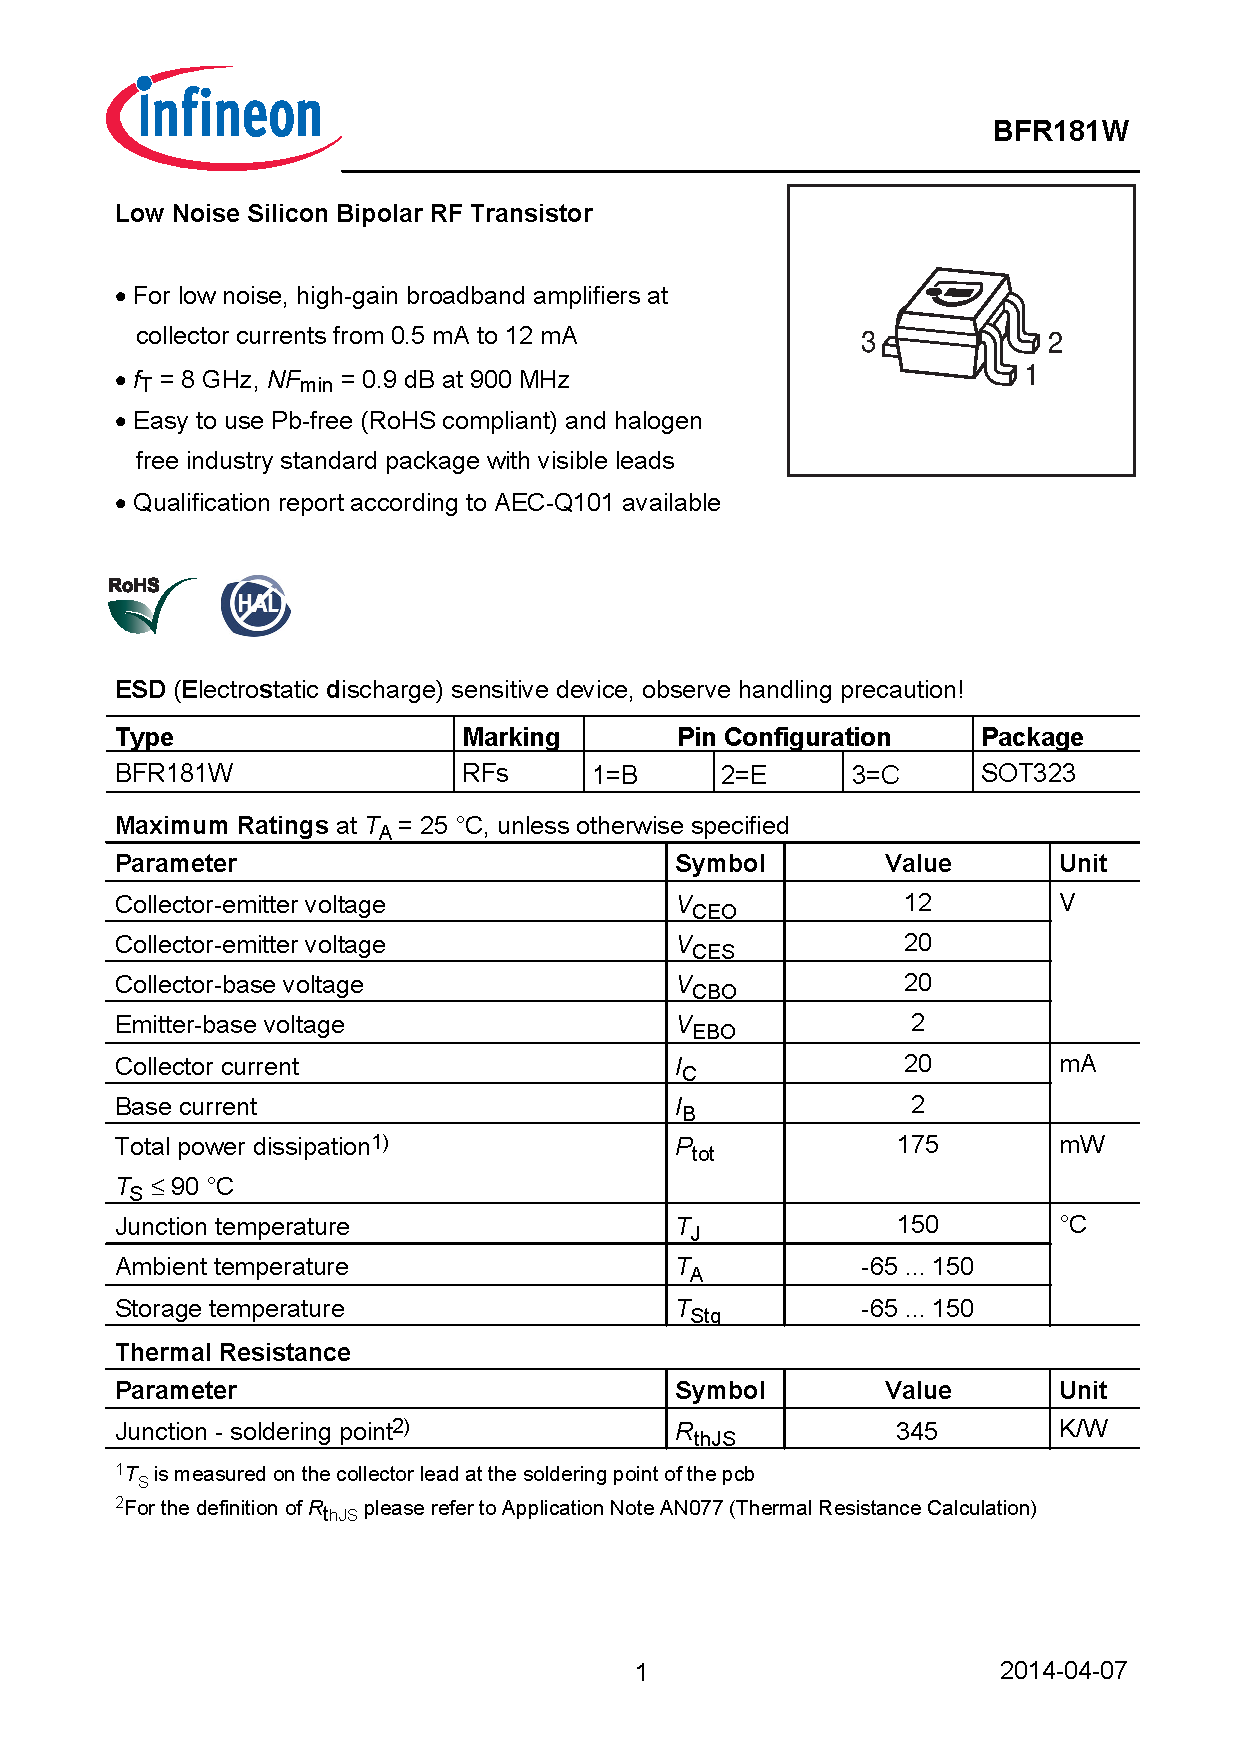
\includepdf[pages=-, pagecommand={\thispagestyle{empty}\setcounter{page}{\thepage}\rfoot{\thepage}}, fitpaper=true, offset=1.0in -1.0in]{C:/Users/Farhad/OneDrive/Desktop/Vorlage neu/GrundlagenPraktikum6G/2_Protokoll/Literature/Infineon_LNA_BFR181W-85922.pdf}
\clearpage
